\documentclass[10pt,aspectratio=169]{beamer}
\usetheme{metropolis}
\usepackage{amsmath,amssymb}
\usepackage{booktabs}
\usepackage{graphicx}
\usepackage{multicol}
\usepackage{caption}

\graphicspath{{figs/}}

\newcommand{\nuc}[1]{\left\|#1\right\|_{\ast}}
\DeclareMathOperator*{\argmin}{arg\,min}

\title{Open-Ended Explorations (Part 3)}
\subtitle{ECE 66200 --- Projects 1 \& 2}
\author{Weiheng Tang}
\date{\today}

\begin{document}
\maketitle

% === 1 ================================================================
\begin{frame}{Roadmap}
Two projects, one theme: \textbf{structural priors improve CNNs}.

\bigskip
\begin{columns}[T]
\column{0.48\textwidth}
\textbf{Project 1 --- DCF}\\[0.3em]
Decomposed Convolutional Filters separate CNN weights into
\emph{shared atoms} + \emph{task-specific coefficients}.

\medskip
\textbf{Part 3:} Exploit this decomposition for
\emph{continual learning} --- sequentially learn multiple
deblurring tasks with zero forgetting.

\column{0.48\textwidth}
\textbf{Project 2 --- OLT}\\[0.3em]
Orthogonal Low-Rank Transformation enforces
\emph{intra-class low rank} + \emph{inter-class orthogonality}
via a nuclear-norm objective.

\medskip
\textbf{Part 3:} Inject the OLT functional as a differentiable
\emph{regularizer} during CNN training.
\end{columns}
\end{frame}

% ======================================================================
%  PROJECT 1 PART 3
% ======================================================================

% === 2 ================================================================
\begin{frame}{P1 Part 3 --- Continual Deblurring: Motivation}
\begin{columns}[c]
\column{0.6\textwidth}
\vspace{20pt}
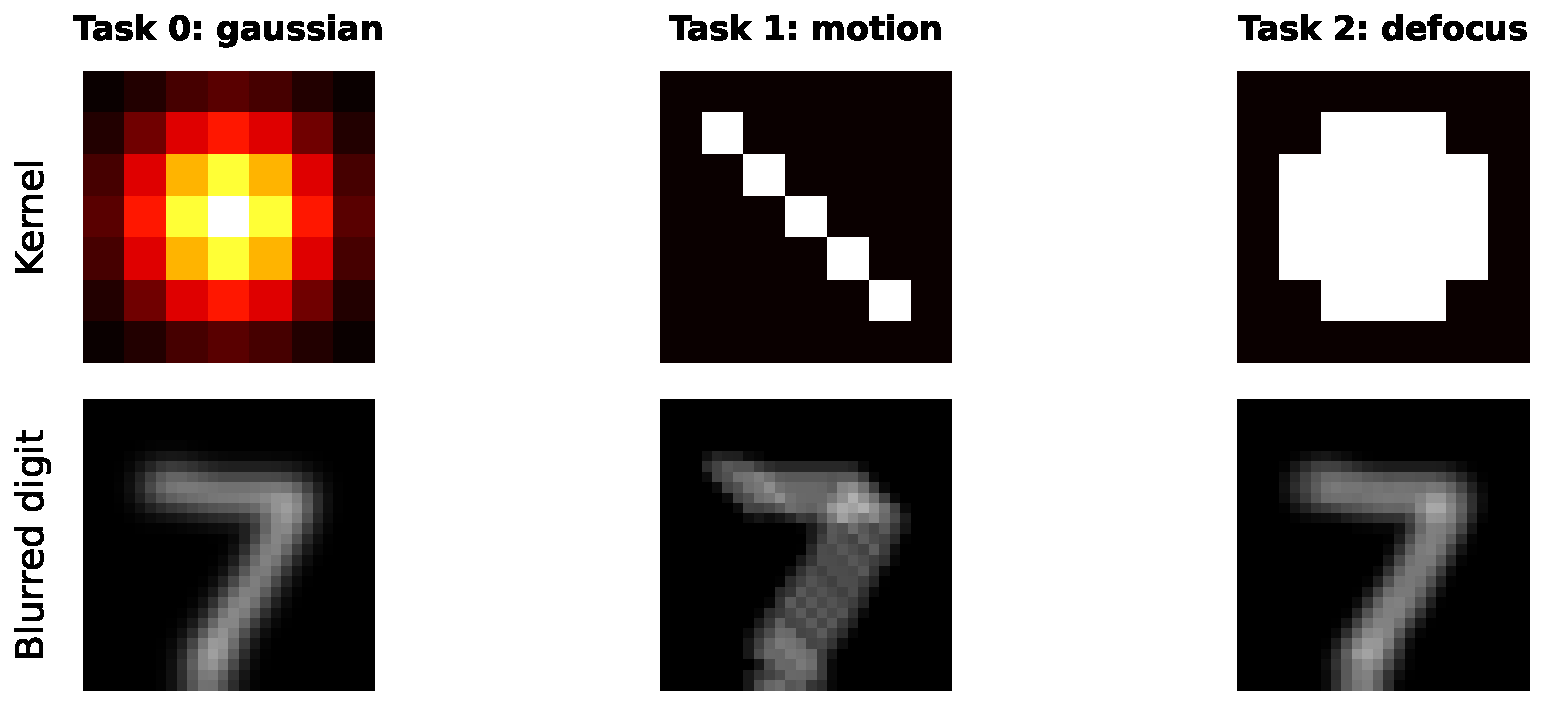
\includegraphics[width=\linewidth]{slide_blur_examples.pdf}
\captionof{figure}{Synthetic blur tasks: PSF kernels (top) and example degraded digits (bottom).}

\column{0.4\textwidth}
\begin{itemize}
\item Sequential training $\Rightarrow$ \textbf{catastrophic forgetting}.
\item Na\"{\i}ve fix: one model per task --- memory grows linearly.
\item DCF splits filters into \emph{shared atoms} + \emph{task-specific coefficients}.
\item \textbf{Idea:} freeze atoms, store only coefficients per new task.
\end{itemize}
\end{columns}
\end{frame}

% === 3 ================================================================
\begin{frame}{P1 Part 3 --- DCF-CL Protocol}
\textbf{Architecture.} Conv/DCF autoencoder ($1\!\to\!32\!\to\!64\!\to\!64$, symmetric decoder), $K\!=\!6$ atoms.

\bigskip
\textbf{Training protocol:}
\begin{enumerate}
\item \textbf{Task 0} (Gaussian blur): train all parameters (atoms + coefficients + decoder). Freeze atoms; store coefficients $\mathbf{a}_k^{(0)}$.
\item \textbf{Task $t>0$}: re-initialise coefficients $\mathbf{a}_k^{(t)}$, BN, and decoder. Train only these; atoms stay frozen. Store $\mathbf{a}_k^{(t)}$.
\item \textbf{Inference on Task $j$}: inject $\mathbf{a}_k^{(j)}$ $\Rightarrow$ \emph{exact} restore (atoms unchanged).
\end{enumerate}

\bigskip
\textbf{Forgetting metric --- Backward Transfer (BWT):}
\[
\mathrm{BWT} = \frac{1}{T{-}1}\sum_{t=1}^{T-1}
\bigl(\mathrm{PSNR}_{T-1,\,t-1} - \mathrm{PSNR}^*_{t-1}\bigr)
\]
Negative BWT $=$ forgetting.\ \ DCF-CL gives $\mathrm{BWT}=0$ \textbf{by construction}.
\end{frame}

% === 4 ================================================================
\begin{frame}{P1 Part 3 --- Results: Forgetting Curves}
\centering
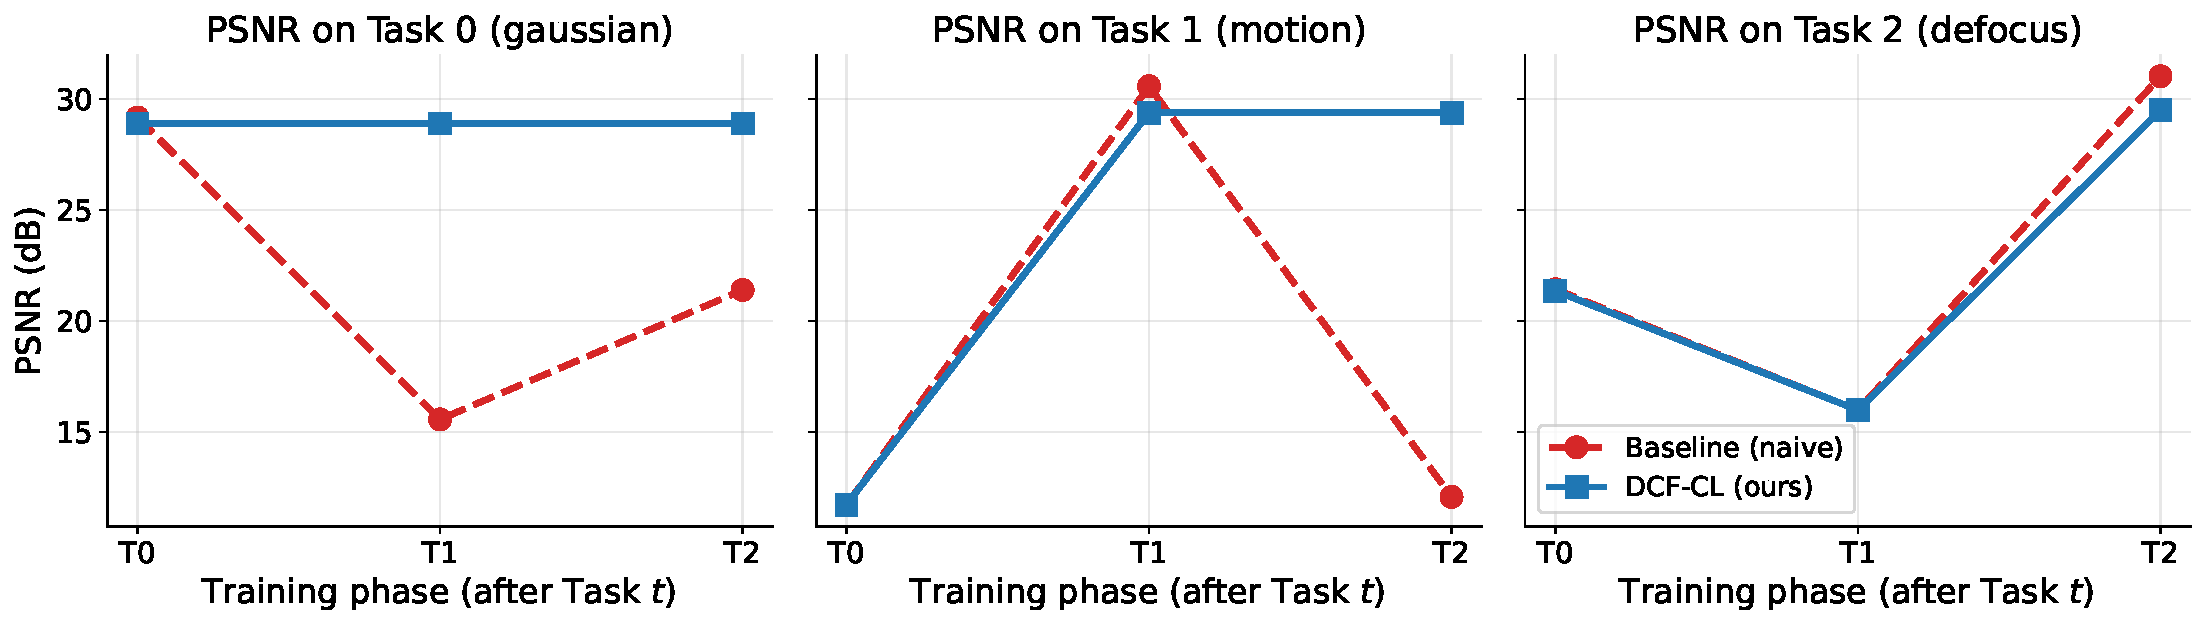
\includegraphics[width=0.95\linewidth]{slide_forgetting_curves.pdf}
\captionof{figure}{PSNR on each task after sequential training phases T0 $\to$ T1 $\to$ T2.}
\smallskip
{\small
\textbf{Baseline (red):} Task 0 drops $29.16 \to 15.57$ dB after Task 1 ($-13.6$ dB).\\
\textbf{DCF-CL (blue):} PSNR locked at peak for every task. BWT: baseline $= -13.1$ dB; DCF-CL $= 0.0$ dB.}
\end{frame}

% === 5 ================================================================
\begin{frame}{P1 Part 3 --- Results: PSNR Heatmaps \& Summary}
    % --- Top Row: Figure ---
    \centering
    % 稍微缩小一点宽度（比如 0.8），给下方的文字留出垂直空间
    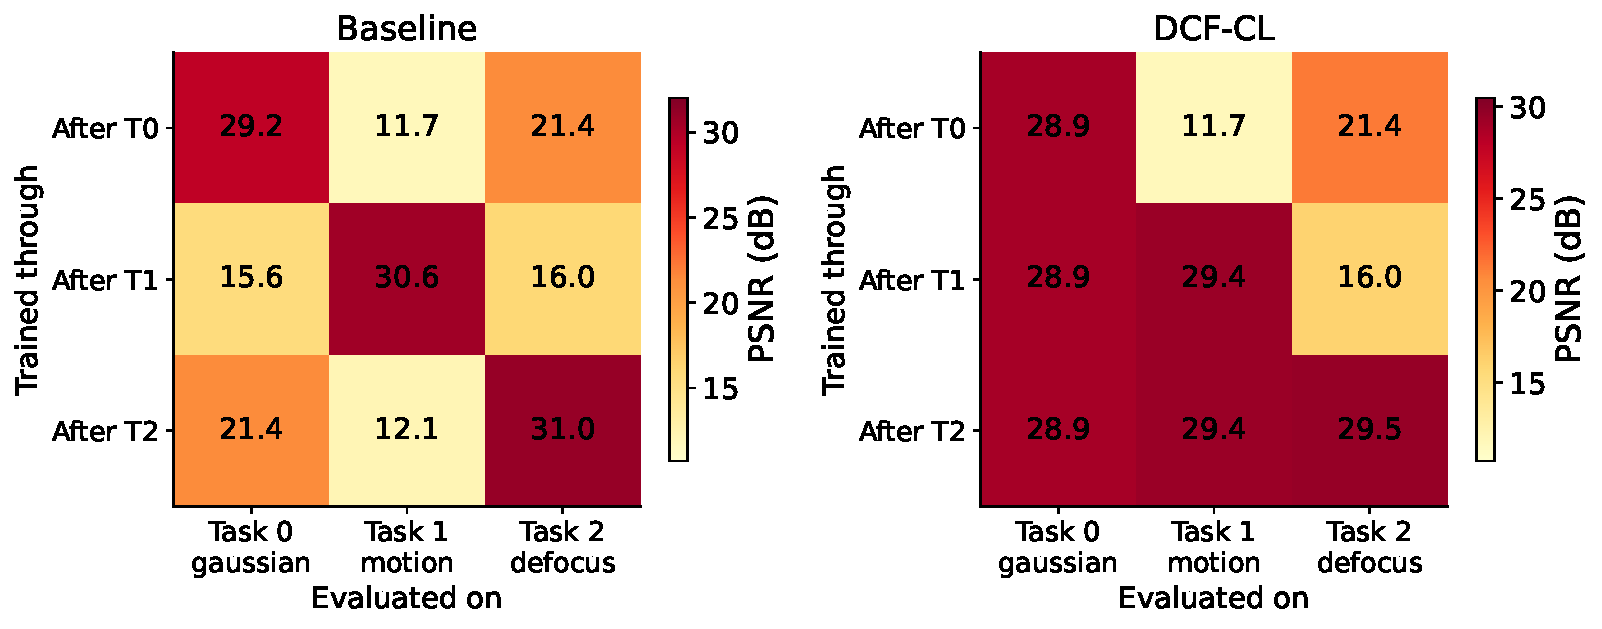
\includegraphics[width=0.85\linewidth]{slide_psnr_heatmaps.pdf}
    \captionof{figure}{PSNR matrix (rows = training phase, cols = evaluation task).}

    \vspace{0.5em} % 调节上下两行之间的间距

    % --- Bottom Row: Table (Left) and Text (Right) ---
    \begin{columns}[t] % 使用 [t] 确保表格第一行和文字第一行对齐
        \column{0.5\textwidth}
        \centering\small
        \begin{tabular}{lcccc}
            \toprule
            & T0 & T1 & T2 & BWT \\
            \midrule
            Baseline & 21.4 & 12.1 & 31.0 & $-13.1$ \\
            \textbf{DCF-CL} & \textbf{28.9} & \textbf{29.4} & \textbf{29.5} & $\mathbf{0.0}$ \\
            \bottomrule
        \end{tabular}

        \column{0.5\textwidth}
        \small
        \vspace{-4em}
        \begin{itemize}
            \item Baseline heatmap: sharp drops below the diagonal.
            \item DCF-CL heatmap: each column \emph{constant} to 4 decimal places.
        \end{itemize}
    \end{columns}
\end{frame}

% === 6 ================================================================
\begin{frame}{P1 Part 3 --- Memory \& Discussion}
\begin{columns}[c]
\column{0.55\textwidth}
\vspace{10pt}
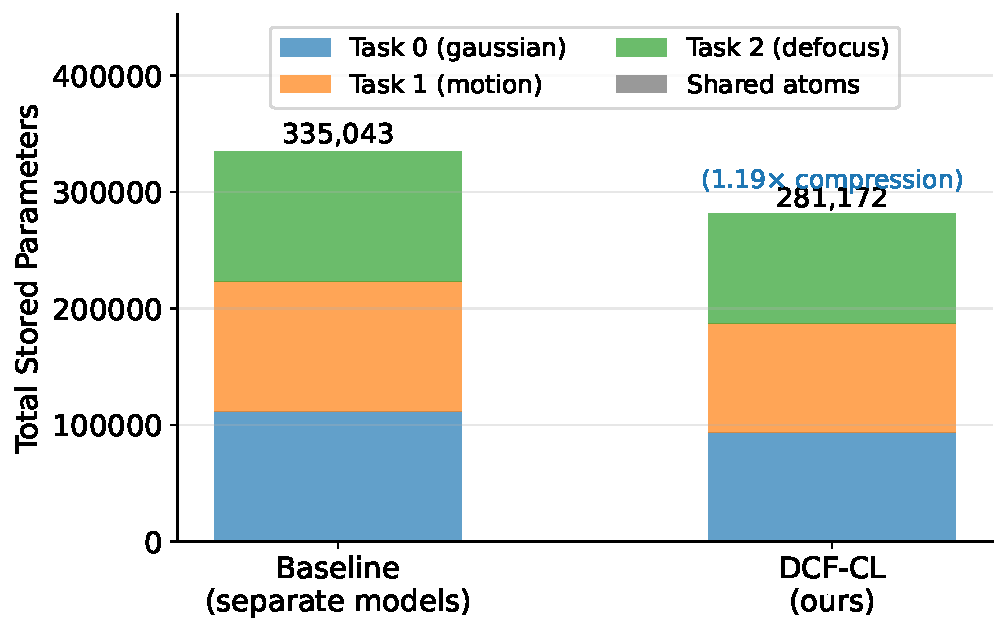
\includegraphics[width=\linewidth]{slide_memory_footprint.pdf}
\captionof{figure}{Memory footprint: baseline vs.\ DCF-CL}

\column{0.4\textwidth}
\begin{itemize}
\item Baseline: $3 \times 111{,}681 = 335$K params.
\item DCF-CL: $162 + 3 \times 93{,}670 = 281$K ($1.19\times$ fewer).
\item Compression is modest because decoder dominates ---
      would grow with deeper/wider encoders or a shared decoder.
\end{itemize}
\end{columns}


\textbf{Key takeaway:}
The DCF decomposition gives \emph{zero forgetting by algebraic construction}, not approximation. Atoms learned on one blur type generalise well enough that later tasks achieve even higher PSNR (29.4--29.5 dB vs.\ 28.9 dB).
\end{frame}

% ======================================================================
%  PROJECT 2 PART 3
% ======================================================================

% === 7 ================================================================
\begin{frame}{P2 Part 3 --- OLT as a CNN Regularizer: Motivation}
\textbf{Context from earlier parts:}
\begin{itemize}
\item OLT works well as a \emph{post-hoc} linear embedding on raw/PCA features
      (Part 1: $+4$ pts over LDA; Part 2: $+16$ pts cross-modality).
\item But applying OLT \emph{after} a frozen CNN hurts ($-1.8$ pts).
\item The linear low-rank prior clashes with nonlinear, ReLU-activated geometry.
\end{itemize}

\bigskip
\textbf{Idea:} instead of retro-fitting OLT, let the network
\emph{co-adapt} its features during training:
\[
\mathcal{L}=\underbrace{\mathrm{CE}(Wf_\theta(x),y)}_{\text{classification}}
\;+\;\lambda\;\underbrace{\frac{1}{|\mathcal{B}|}\!\left(
\sum_c\nuc{F_c}-\nuc{F}\right)}_{\text{OLT regularizer}}
\]
Differentiable through PyTorch's SVD --- gradient flows to $\theta$.
\end{frame}

% === 8 ================================================================
\begin{frame}{P2 Part 3 --- Why This Should Work}
The two loss terms are \textbf{complementary}:

\bigskip
\begin{columns}[T]
\column{0.48\textwidth}
\textbf{Cross-entropy}
\begin{itemize}
\item Assigns samples to correct classes.
\item Says nothing about \emph{geometry} between classes.
\item Two classes can overlap heavily as long as a linear boundary separates them.
\end{itemize}

\column{0.48\textwidth}
\textbf{OLT regularizer}
\begin{itemize}
\item Compresses each class to a low-rank manifold ($\nuc{F_c}$ small).
\item Pushes class subspaces toward orthogonality ($\nuc{F} \to \sum_c\nuc{F_c}$).
\item Provides implicit geometric margin --- robust to within-class variation (e.g.\ rotation).
\end{itemize}
\end{columns}
\end{frame}

% === 9 ================================================================
\begin{frame}{P2 Part 3 --- Results: $\lambda$ Sweep}
\centering
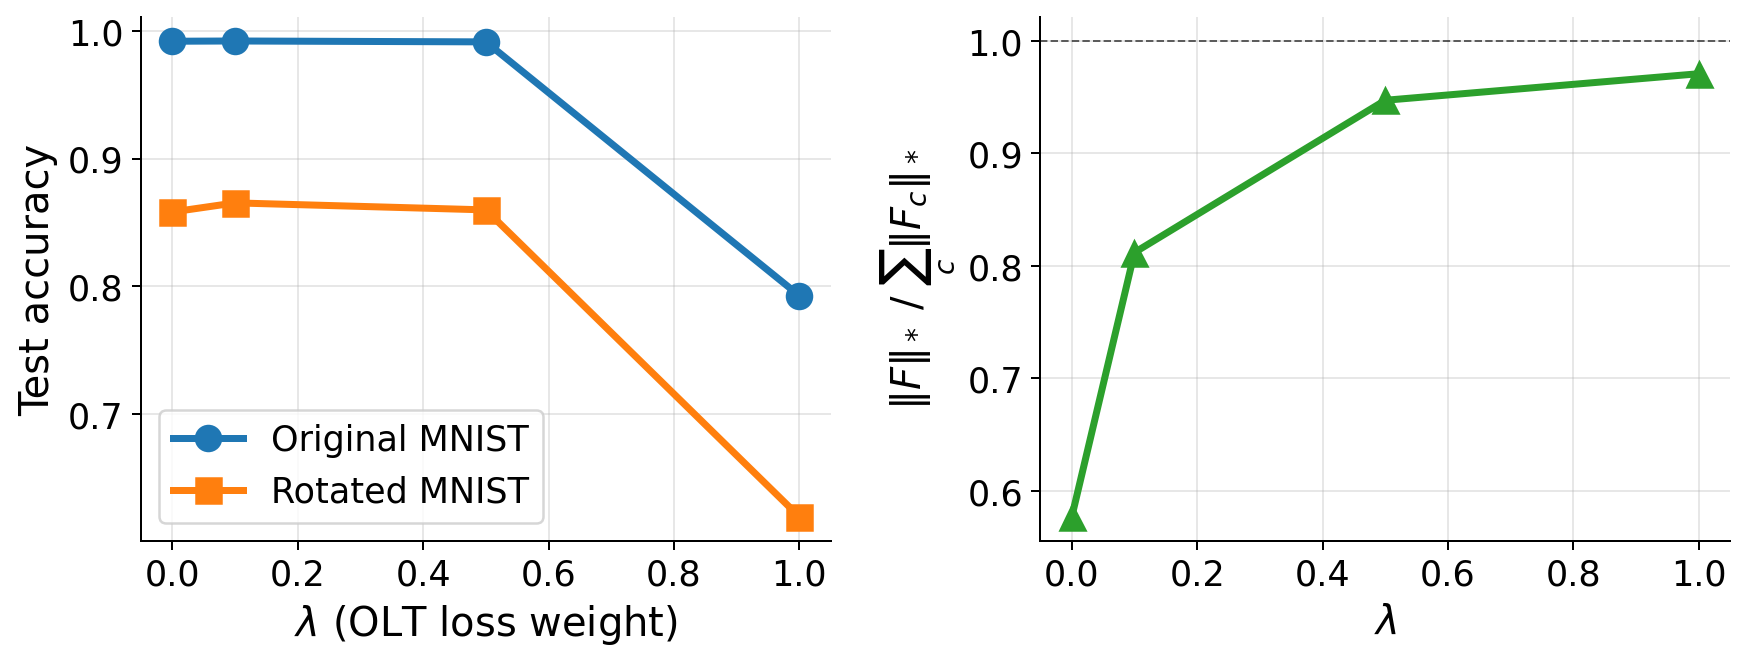
\includegraphics[width=0.75\linewidth]{slide_lambda_sweep.png}
\captionof{figure}{Left: accuracy vs.\ $\lambda$. Right: feature-subspace orthogonality (higher = more orthogonal).}
\vspace{0.3em}
\small
\begin{tabular}{ccccc}
\toprule
$\lambda$ & Orig acc & Rot acc & $r$ (orthogonality) & Regime \\
\midrule
$0.0$ & $0.9919$ & $0.8582$ & $0.577$ & baseline \\
$\mathbf{0.1}$ & $\mathbf{0.9921}$ & $\mathbf{0.8653}$ & $0.812$ & \textbf{beneficial} \\
$0.5$ & $0.9914$ & $0.8598$ & $0.947$ & saturated \\
$1.0$ & $0.7926$ & $0.6195$ & $0.971$ & collapse \\
\bottomrule
\end{tabular}
\end{frame}

% === 10 ===============================================================
\begin{frame}{P2 Part 3 --- Three Regimes}
\begin{description}
\item[Regime 1 ($\lambda\!=\!0.1$): Beneficial regularization.]
  CE still dominates; OLT nudges features toward orthogonality
  ($r: 0.58\!\to\!0.81$).
  Rotated accuracy $+0.7$ pts --- orthogonal subspaces absorb
  rotation-induced variance.

\item[Regime 2 ($\lambda\!=\!0.5$): Geometric saturation.]
  Near-perfect orthogonality ($r\!=\!0.95$) but accuracy stagnates
  at baseline. OLT consumes representational capacity;
  gain from geometry $\approx$ loss of flexibility.

\item[Regime 3 ($\lambda\!=\!1.0$): Collapse.]
  OLT overwhelms CE. Features are perfectly orthogonal but
  semantically arbitrary: $79\%$ clean, $62\%$ rotated.
  Nuclear norm shapes \emph{how} features cluster, not
  \emph{which} features belong where.
\end{description}

\bigskip
Analogous to $L_2$ weight decay: a small structural penalty helps;
too much underfits. OLT regularizes \emph{feature geometry}, not
weight magnitudes.
\end{frame}

% === 11 ===============================================================
\begin{frame}{Connecting Themes}
Both Part 3s demonstrate: \textbf{structural priors are most powerful
when they participate in learning.}

\bigskip
\begin{columns}[T]
\column{0.48\textwidth}
\textbf{Project 1: DCF $\to$ Continual Learning}
\begin{itemize}
\item Atoms/coefficients split $\Rightarrow$ freeze atoms, swap coefficients.
\item Zero forgetting by construction (BWT $= 0$).
\item Prior shapes the \emph{architecture} so learning is modular.
\end{itemize}

\column{0.48\textwidth}
\textbf{Project 2: OLT $\to$ Feature Regularizer}
\begin{itemize}
\item Nuclear-norm functional $\Rightarrow$ differentiable loss term.
\item Post-hoc OLT \emph{hurts} ($-1.8$ pts); end-to-end \emph{helps} ($+0.7$ pts).
\item Prior shapes the \emph{loss} so features co-adapt.
\end{itemize}
\end{columns}

\bigskip
\centering
\fbox{\parbox{0.85\textwidth}{\centering
\textbf{Common lesson:} A geometric/structural prior imposed \emph{after}
training fights the learned representation.\\
Integrated \emph{during} training, it guides the network to
representations that are both accurate and well-structured.}}
\end{frame}

\end{document}
